\section{Test description}
\label{section:test_description}

In this section I will describe which metrics I am going to use to compare the different algorithms. Having specified these I will describe the tests in detail.

\subsection{Metrics}

The metrics I will measure in the tests will be 
\begin{description}
\item[Number of hops:] The number of hops from the source to the sink. For this I will measure the maximum number of hops, the minimum number of hops, as well as the average. I feel the number of hops is the most important metric, since it both details how many nodes that have to expend energy before the message arrives at the node, how long it takes for the message to arrive at its destination, and how great the risk is that the network topology will make it impossible for the message to arrive (assuming, of course, that the message could arrive when it was sent).

\item[Time:] The amount of time spent sending the message from the source to the sink. I will likewise measure the maximum, minimum and average time spent. It is clear that the faster a message arrives at its sink, the better.

\item[Number of misses:] The ratio of timeouts compared to the number of sent messages. This will apply whether we are using UDP or TCP. \todo{make this more precise}

\item[Percentages of successfully arrived messages:] While most\todo{qualify/quantify this} routing algorithms guarantees that the message will always arrive, this is not always the case. The best example of a routing algorithm that does not have this guarantee is the greedy routing algorithm (see Section~\ref{greedy} p. \pageref{greedy}). Also, since we are trying to simulate mobile nodes with limited energy storage, critical parts of the topology may be fail, making it impossible for the message to arrive.
\end{description}

For the number of hops, the amount of time and number of misses I will record the maximum, the minimum and the average value. The main value for comparison will be the average value, but I feel that recording both the maximum and the minimum values will give me a view of both the extremes, but also gives me additional information about the average.

\subsection{Input parameters}
\label{input_parameters}
In order to perform the tests I will need to define the parameters and their range for the different tests.
\begin{description}
\item[Movement model:] The topology is clearly going to be influenced by the way that the nodes move, therefore it would be interesting to test out several models, to see the strengths and weaknesses of the different routing algorithms.

\item[Routing Algorithms:] 

\item[Amount and data-transmission type:] In real world situations there will be different levels of traffic on the network, and therefore to test it we must likewise simulate these differences. The choice of transmission protocol is also important. Applications that uses the UDP protocol are less likely to cause congestion in the network, compared to applications that uses the TCP protocol.

\item[Size of the simulation area:] The size of the simulation area has a direct influence on how far apart the nodes can move and how many nodes are needed for a given node density. Everything else being equal, a larger simulation area will make the network less robust.

\item[Number of nodes:] It is clear that denser node distribution, everything else being equal, will give a more robust network,

\item[Percentage of nodes failing/leaving the network:] Since we are dealing with a \ac{manet}, it is clear that a nodes may leave the network or fail (either due to equipment failure or lack of power). 
\item[Percentage of nodes entering the network:] In a \ac{manet} we have to assume that nodes can enter the network.
\end{description}


\subsection{Actual parameters}
As I have now detailed in section~\ref{input_parameters} which parameters it would be useful to vary, I will in this subsection detail the actual value of the different parameters. 

\begin{itemize}
\item[Movement models:] DisasterArea \cite{disasterArea} and Gauss-Markov \cite{MobilityAdHocResearch}. In practise I will create a trace using the BonnMotion tool \cite{toilers} use to create the movement files which can then be imported into ns-2.
\item[Amount and Data-transmission type:] 500 kB, 1024 kB, 5120 kB, 20480 kB (TCP), 500 kB, 5120 kB, 51200 kB (UDP)
\item[Size of simulation area:] 500 by 500 units and 1000 by 1000 units
\item[Routing algorithms:] GOAFR \cite{gopher}, GOAFR+ \cite{gopher+}, Greedy \cite{gopher}, DSDV \cite{DSDV}
\item[Number of nodes:] 500, 750, 1000
\item[Nodes failing:] 0\%, 10\%, 40\%
\item[Nodes entering:] 0\%, 15\%
\end{itemize}

Not all combinations are going to be tried, since this would create far too many tests to feasibly to test or analyse. However, some of these are going to be combined. For instance it would be preferable to do different data-transmissions during the life time of the network.\todo{finish this up}

\subsection{Routing algorithm description}
In this description of the chosen routing algorithms, I will assume by default that there exists a path from the source to the sink, and if needed I will detail how the algorithm handles the cases where no such path exists.

\subsubsection{GOAFR and GOAFR+}

\tikfig{gopher}{}\todo{redo the figure so there is actual a point}

GOAFR \cite{gopher} (Greedy Other Adaptive Face Routing) and GOAFR+ \cite{gopher+} (a refinement on GOAFR) are multi-stage geometrical algorithms. The algorithms are based on Greedy routing (see section~\ref{greedy} on p. \pageref{greedy}) and Adaptive Face Routing, with an adaptive ellipse $\epsilon$ as the boundary for the message. The description in the following paragraphs uses information from \cite{gopher}.

As an integral part of the algorithm, GOAFR includes $\epsilon$ that that the message has to keep inside. $\epsilon$ is created so that its forci are node $s$ and node $t$, and so that its longest axis starts out being $2 * |\overline{st}|$. Using the formula for forci
\eqa{
F = \sqrt{j^2 - n^2}
}
where $F$ is the distance from each forci to the centre, $j$ is the semi-major axis (major radius), and $n$ is semi-minor axis (minor radius) so
\eqa{
F &=& \sqrt{j^2 - n^2}\\
\frac{|\overline{st}|}{2} &=& \sqrt{j^2 - n^2}\\
\left(\frac{|\overline{st}|}{2}\right)^2 &=& j^2 - n^2\\
n^2 &=& j^2 - \left(\frac{|\overline{st}|}{2}\right)^2\\
n &=& \sqrt{j^2 - \left(\frac{|\overline{st}|}{2}\right)^2}\\
}
which gives us the minor axis. Depending on the execution of GOAFR the major axis of $\epsilon$ might grow, as detailed in the next two paragraphs.

Greedy routing works as described in section~\ref{greedy}, except that when it arrives at a local minimum, the algorithm begins to apply the Adaptive Face routing. If the greedy algorithm sends the message beyond the bound of $\epsilon$, then the longest axis of $\epsilon$ is doubled.

Adaptive Face routing is based on the right-hand rule, introduced in section \ref{right-hand rule} p. \pageref{right-hand rule}, which here is applied to traverse a face, until you either encounter the sink, or another face that lies closer to the sink than the one you are currently traversing. Of course, there is no guarantee that the face you are traversing is not the outer-face (the face not being bounded by the nodes) and therefore might be a dead-end or a detour (see figure \todo{make figure}). If the message encounters $\epsilon$ for the first time, then the message reverses direction and tries to traverse the face in the other direction. If the message encounters $\epsilon$ for the second time, then the longest axis of $\epsilon$ is doubled and the algorithm starts over. There exist several different criteria for when the face routing stops -- either when the line-segment $\overline{st}$ is passed by the message, or when the messages arrives back at the node where the face routing started.

Surmising GOAFR works by:
\begin{enumerate}
\item Using Greedy routing until this is no longer feasible or the sink has been found
\item Using Adaptive Face routing to either find the node closest to the sink and then use greedy routing
\end{enumerate}
All the while using $\epsilon$ to limit the spreed of the message, but expanding it cautiously.

GOAFR+ works similarly to GOAFR, with th difference being the introduction of 2 variables $p$ and $q$. While doing the adaptive face routing from the local minimum node $x$, the algorithm keeps track of how many nodes encountered that are closer to the sink than $x$ in the variable $p$ and how many are farther away in the variable $q$.
A special action is then taken if
\begin{enumerate}
\item If the message arrives at the edge of $\epsilon$ for the first time, then the message turns back and explores the face in the other direction. 
\item If the message arrives at the edge of $\epsilon$ for the second time, and no nodes have been found to be closer to the sink than $x$, then the major axis of $\epsilon$ is doubled. Otherwise the message is sent to the node closest to the sink and the greedy routing is resumed.
\item If at any point $p > \rho q$, where $\rho$ is a constant defined before routing starts, then route the message to the node closest to the sink and begin greedy routing again.
\end{enumerate}

Both GOAFR and GOAFR+ has proved to be theoretical asymptotically worst-case optimal and average-case efficient. Due to space demands I will not try to prove these claims here, but will instead refer the interested reader to \cite{gopher+} and \cite{gopher}.

\subsubsection{Mobility models}


blah blah



\subsection{Limited-range spanner tests}
\label{section:test_desc_spanners}
In this section I will detail how I have chosen to set up the limited-range spanner tests for the three different graphs: non-planar, the \acp{gabe} and the \acp{rng}.

\subsubsection{Creation of the graphs}
It is clear that we must create several graphs of several different number of nodes, as it otherwise is impossible to gain a proper perspective on how well the \ac{gabe} and the \ac{rng} stack up against the non-planar graph.

Because of this I have decided on creating graphs with 8 different number of nodes: 100, 250, 500, 1000, 2500, 5000, 7500 and 10000 nodes. I feel this would give me a big enough spread, while still being feasible to calculate in a reasonable amount of time. Since we are dealing with limited-range spanners, the value of the node density and the radio-range of the nodes becomes important. Different densities and radio-ranges would heavily influence the outcome of the results, as a high node density/radio-range would favour the non-planar graph over the two other graph types, while a low density/radio-range would create heavily disconnected graphs in all three cases. Since having many disconnected graphs would make testing difficult, I have tried to find combination that would give me a low number of graphs pr. node-set, while still keeping the density low. From several experiments this let me to a density of 0.01 nodes pr. square unit and a radio range of 20 units, and make the space the nodes are placed over a function of the number of nodes. Specifiably, if we let $x$ be the length of the sides in a square and $num$ be the number of nodes, then we have that the density is
\begin{eqnarray}
\frac{num}{x^2} &=& 0.01 \\
num &=& 0.01 * x^2 \\
num * 100 &=& x^2 \\
x &=& \sqrt{100 * num}  
\end{eqnarray}

\subsubsection{Tests to be performed}
In order to check the limited-range spanner for the three graphs, I will randomly pick two different nodes, a \emph{node-pair}, that are connected in the non-planar graph and record the shortest number of hops (the \emph{Unit distance}), as well as the shortest distance between the two nodes. I feel both values are worth finding, as the number of hops is directly applicable to \acp{manet}, while the distance is interesting from a more theoretical perspective, and will therefore also be recorded. 

I will do this for all three types of graphs, and record whether or not a path exist between the node-pair in the \ac{gabe} or the \ac{rng}. If it is indeed the case that there are cases where the two alternative planar graphs removes paths, that would create an element of risk by employing them, instead of the non-planar graph.

\subsubsection{Analysis}

For each node-pair tested for the graphs I will find the total distance passed, the average distance and the average maximum and minimum distance for all the tests\footnote{I feel it is necessary to use the average since there may be outliers that easily could skew the results}. Likewise I will find the total number of hops, the average number of hops and the average maximum and minimum number of hops. Since one of the advantages of the \ac{gabe} and the \ac{rng} is that they have fewer neighbours, I will also find the total number of neighbours, the average, max- and minimum number of neighbours. I will also include the average number of connected components\todo{Should I define this?} 

\todo{Decide whether you think the size of the graph is important and why it should be mentioned} 

\subsubsection{Size of the test}
In order to make the tests more fair I decided to randomly generate 500 different node-sets for each of the sizes. Each node-set is then used to generate the three types of graph. For each node-set I then generate 100 node-pairs. I feel that this will give me an reasonable amount of data to analyse, while still being computable for the larger number of nodes.


\subsubsection{Source code and test data}
The python scrips I used to generate and tests the graphs can be found at \texttt{src/spanner/spanner\_check.py} along with the data (see the README for explanation) and \texttt{src/spanner/graph\_support} in the GitHub repository refereed to in section~\ref{section:source_code} on p.~\pageref{section:source_code}. All requirements in the code is mentioned in the README file.\\

Due to the sheer size of the test data (well in excess of 10 GB), I am unable to upload all of it to my repository, and I have therefore only uploaded the node-sets, since all the graphs will be able to be created from them (though sadly not the node pairs).

%\tikgraph{avg_neigh}{caption}

\begin{figure}
\centering
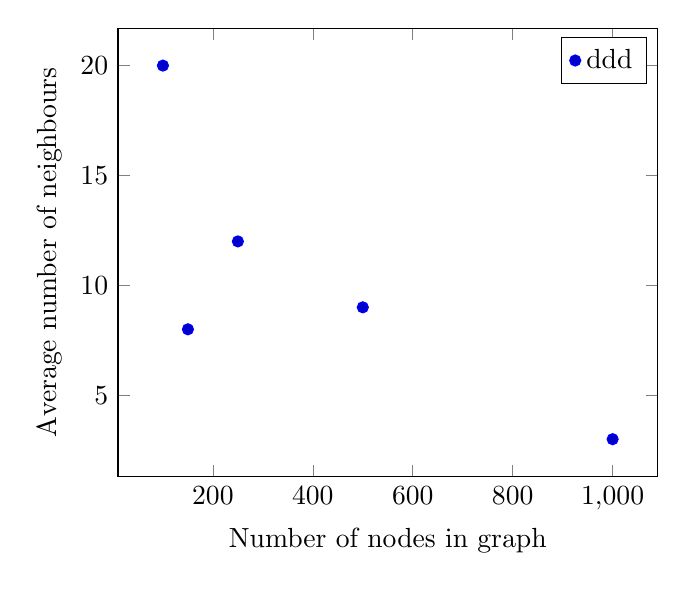
\begin{tikzpicture}
\begin{axis}[xlabel=Number of nodes in graph, ylabel=Average number of neighbours]
\addplot+[only marks] coordinates{
(100, 20) (150, 8) (250, 12) (500, 9) (1000, 3)
};
\legend{ddd}
\end{axis}
\end{tikzpicture}
\caption{Example}
\end{figure}

\hide{
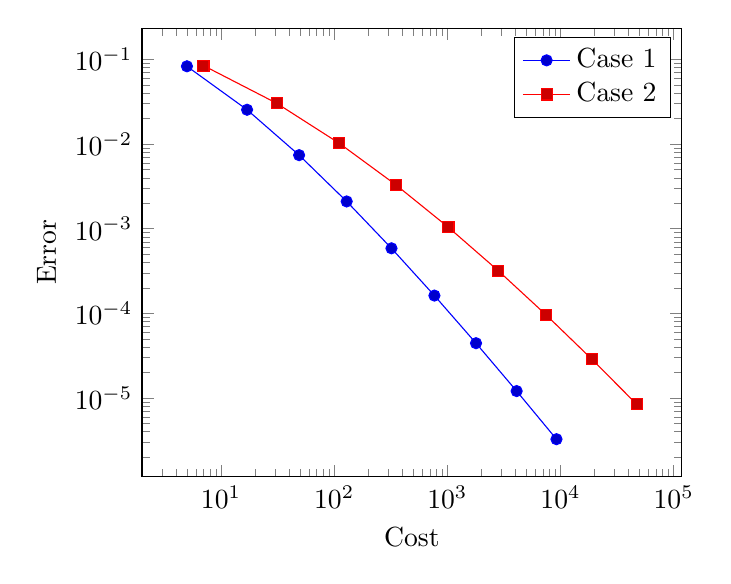
\begin{tikzpicture}
\begin{loglogaxis}[xlabel=Cost,ylabel=Error]

\addplot coordinates {
(5,
8.31160034e-02)
(17,
2.54685628e-02)
(49,
7.40715288e-03)
(129,
2.10192154e-03)
(321,
5.87352989e-04)
(769,
1.62269942e-04)
(1793, 4.44248889e-05)
(4097, 1.20714122e-05)
(9217, 3.26101452e-06)
};
\addplot coordinates {
(7,
8.47178381e-02)
(31,
3.04409349e-02)
(111,
1.02214539e-02)
(351,
3.30346265e-03)
(1023, 1.03886535e-03)
(2815, 3.19646457e-04)
(7423, 9.65789766e-05)
(18943, 2.87339125e-05)
(47103, 8.43749881e-06)
};
\legend{Case 1,Case 2}
\end{loglogaxis}
\end{tikzpicture}
\caption{A larger example}
\end{figure}
}
